\documentclass[14pt]{article}
\usepackage[a4paper, margin=1in]{geometry}
\usepackage[ngerman]{babel}
\usepackage{graphicx}
\usepackage{titlesec}
\usepackage{fancyhdr}
\usepackage{setspace}

\usepackage{fancyvrb}


\usepackage{listings}
\usepackage{color}

\definecolor{dkgreen}{rgb}{0,0.6,0}
\definecolor{gray}{rgb}{0.5,0.5,0.5}
\definecolor{mauve}{rgb}{0.58,0,0.82}

\lstset{frame=tb,
  language=sh,
  aboveskip=3mm,
  belowskip=3mm,
  showstringspaces=false,
  columns=flexible,
  basicstyle={\small\ttfamily},
  numbers=none,
  numberstyle=\tiny\color{gray},
  keywordstyle=\color{blue},
  commentstyle=\color{dkgreen},
  stringstyle=\color{mauve},
  breaklines=true,
  breakatwhitespace=true,
  tabsize=3
}


% Customizing section headers
\titleformat{\section}{\large\bfseries}{\thesection.}{0.5em}{}
\titleformat{\subsection}{\normalsize\bfseries}{\thesubsection.}{0.5em}{}

% Header and footer
\pagestyle{fancy}
\fancyhf{}
\lhead{Kantonsschule Solothurn}
\rhead{Schwachstellenanalyse: SEB}
\cfoot{\thepage}

% Line spacing
\onehalfspacing

\begin{document}

% Cover Page
\begin{titlepage}
    \centering
    \vspace*{5cm}
    {\huge\bfseries Schwachstellenanalyse: Umgehung des Safe Exam Browser mittels KVM-over-IP\par}
    \vspace{1.5cm}
    {\large Alim Weber\par}

    {\large \today\par}
\end{titlepage}

% Executive Summary
\newpage
\section*{Management Summary}
\addcontentsline{toc}{section}{Management Summary}
Lockdown-Browser wie der Safe Exam Browser (SEB) gelten als gängige Sicherheitsmassnahme zur Betrugsprävention in digitalen Prüfungsumgebungen. Sie verhindern durch softwareseitige Sperren den Zugriff auf unerlaubte Ressourcen und Anwendungen. Dieses Whitepaper zeigt jedoch auf, dass solche Systeme durch externe hardwarebasierte Angriffe umgangen werden können.

Im Rahmen der Analyse wurde demonstriert, wie die SEB-Sicherheitsmechanismen mittels einer KVM-over-IP-Lösung vollständig unterlaufen werden können. Diese Technik erlaubt es, ein Prüfungsgerät aus der Ferne zu steuern, ohne dass die Lockdown-Software die Kontrolle registriert oder unterbindet. Der Angriff funktioniert unabhängig vom Betriebssystem und ist nicht durch klassische Software-Updates behebbar.

Die Erkenntnisse verdeutlichen, dass Prüfungsorganisationen bei der Absicherung digitaler Prüfungen neben softwarebasierten Lösungen auch physische und netzwerkbezogene Sicherheitsaspekte stärker be- rücksichtigen müssen. Ohne zusätzliche Massnahmen zur Härtung der Systemumgebung bleibt das Risiko für unerwünschte Manipulationen bestehen.

% Table of Contents
\newpage
\tableofcontents

% Introduction
\newpage
\section{Einführung}
Der Safe Exam Browser (SEB) ist eine von der ETH Zürich entwickelte Lockdown-Software, die während Prüfungen den Zugriff auf unerlaubte Ressourcen und Anwendungen auf dem Prüfungsgerät unterbindet. Ziel ist es, durch die Einschränkung von Funktionen wie dem Zugriff auf das Internet (z. B. Google, ChatGPT oder ähnliche Hilfsmittel) Betrugsversuche während digitaler Prüfungen deutlich zu erschweren. Seit der Einführung des SEB gab es zahlreiche Versuche, die Integrität dieser Sicherheitslösung zu unterlaufen. In der Regel konnten diese Schwachstellen durch zeitnahe Software-Updates behoben werden. Dieses Whitepaper beschreibt jedoch einen alternativen Angriffsvektor, der sich weder durch ein einfaches Update noch durch den Wechsel zu einer anderen Lockdown-Software vollständig eliminieren lässt.

% Problem Statement or Background
\section{Problemstellung}
Trotz der weitreichenden Sicherheitsmassnahmen von Lockdown-Browsern wie dem Safe Exam Browser (SEB) besteht weiterhin das Risiko, dass Prüflinge alternative Wege finden, um Prüfungsregeln zu umgehen und unerlaubte Hilfsmittel zu verwenden. Während bekannte Angriffsvektoren oftmals durch regelmässige Software-Updates adressiert werden können, existieren Methoden, die unabhängig von der jeweiligen Lockdown-Software sind und auf tieferliegende Schwachstellen im Gesamtsystem abzielen. Diese weniger offensichtlichen Angriffspunkte gefährden die Integrität von Online-Prüfungen und stellen sowohl Bildungseinrichtungen als auch Softwareentwickler vor neue Herausforderungen.

Dieses Whitepaper identifiziert und analysiert eine dieser bisher wenig beachteten Schwachstellen und zeigt auf, weshalb klassische Sicherheitsmechanismen hier an ihre Grenzen stossen.

\section{Methodik}

Die in diesem Whitepaper vorgestellte Methode zur Umgehung der SEB-Restriktionen basiert auf dem Einsatz einer KVM-over-IP-Lösung. KVM-over-IP-Systeme ermöglichen es, ein Gerät vollständig von einem anderen System aus zu steuern und gleichzeitig den Video-Feed des Zielgeräts zu überwachen. Ein Prüfling könnte so externe Steuerungs- und Überwachungsmechanismen nutzen, ohne dass dies vom Safe Exam Browser erkannt wird.

Für die Umsetzung wurde ein KVM-over-IP-System auf Basis eines Raspberry Pi Zero 2 W realisiert. Der Raspberry Pi wurde so programmiert, dass er als USB-Gerät agiert und Tastatur- sowie Maus-Inputs an das Prüfungsgerät (ein Lenovo ThinkPad T530) emuliert.

Der Video-Feed des Prüfungsgeräts wurde über einen Mini-DisplayPort-zu-HDMI-Adapter und eine Capture Card in einen externen Computer eingespeist. Zur Weiterleitung des Bildsignals wurde der Video-Stream mit Hilfe von \verb+mjpeg_streamer+ kodiert und auf einer webbasierten Steuerkonsole angezeigt, die sowohl das Live-Video als auch Eingabemöglichkeiten für Tastatur- und Mausbefehle bot.

Für die vollständige Remote-Steuerung wurde das System zusätzlich über einen Fernwartungsdienst (z. B. Anydesk) für weitere externe Geräte zugänglich gemacht. Auf diese Weise konnte der Prüfungs- rechner aus der Ferne bedient und manipuliert werden, ohne dass der SEB eine Abweichung vom vorgesehenen Lockdown-Modus detektieren konnte.

Es wurde ebenfalls evaluiert, dass bei einer einfachen Nutzung des „Zwischengeräts“ (externer Computer) im direkten Umfeld des Prüfungsgeräts die physische Manipulation (z. B. zusätzliche Kabel) leicht auffallen könnte. Daher zielt der vollständige Angriff darauf ab, die Steuerung vollständig auf ein externes Endgerät zu verlagern. 

\begin{figure}[h!]
	
	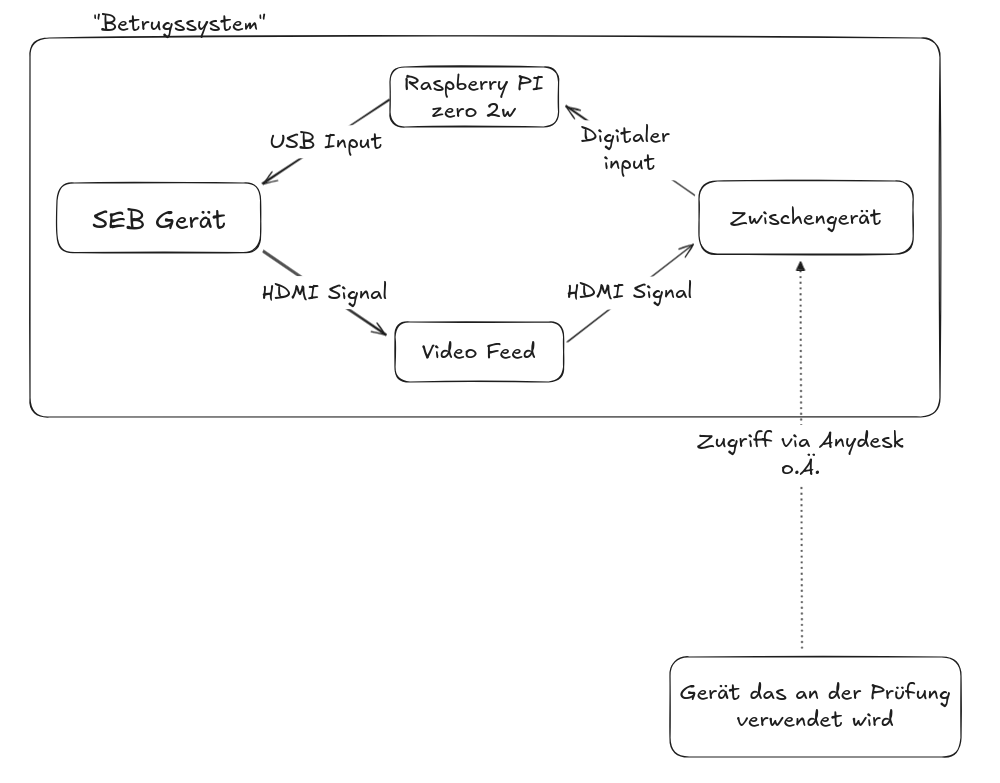
\includegraphics[width=\linewidth]{./images/schematic1.png}
	\caption{Schematische Abbildung des Betrugsaufbaus}

\end{figure}

\subsection{Limitationen und mögliche Schwierigkeiten}

Auch diese Attacke ist nicht unfehlbar, und so sind unten einige Schwierigkeiten aufgeführt.

\begin{itemize}
	\item Weil es sich bei diesem Angriffsvektor um eine Art der "Externalisierung" handelt, die zwingend auf Netzwerk Zugriff beruht, kann bei Fehlen eben dieses Netzzugriffs nicht auf diese Attacke zurückgegriffen werden. 

	\item Der Prüfling Muss zwingend mindestens drei Geräte Besitzen, eines das er an der Prüfung benutzt, eines das den Video-Feed streamt und eines auf dem der SEB tatsächlich läuft. 
	
	\item Die Konfiguration von Input Geräten die man per Fernzugriff steuern kann, ist Herausfordernd und nicht trivial.

\end{itemize}



\newpage
% Proposed Solution / Approach
\section{Lösungsansätze}

Allem voran ist diese Art des Betrugs sehr aufwendig, und wohl kaum grossflächig anwendbar, allerdings dürfen solche Möglichkeiten nicht unterschätzt werden. Die Lösungsansätze die uns zur Verfügung stehen, lassen sich in zwei Kategorien einordnen: 

\begin{enumerate}
\item Traditionelle Methoden
\item Strengere Einschränkungen während Prüfungen
\item Eine Überarbeitung der Art des Prüfens
\end{enumerate}

\subsection{Traditionelle Methoden}
Unter den Traditionellen Methoden verstehen sich z.B. herumlaufende Lehrer, Abschreibwände etc. Während sich letztere erübrigen ist ersteres sehr wichtig und wird auch immer wieder von den Betreibern solcher Lockdown Lösungen empfohlen. Weiter kann ein Prüfling überführt werden der keine SEB Log Files vorweisen kann.


\subsection{Strengere Einschränkungen}

Technische Massnahmen zur Verschärfung der Prüfungsumgebung erscheinen auf den ersten Blick als die naheliegendste Option, sind jedoch langfristig nur eingeschränkt wirksam. Aufgrund der hardwarebasierten Natur der hier vorgestellten Angriffsmethode greifen klassische Lockdown-Lösungen – einschliesslich alternativer Browser oder Sperrsoftware – nicht mehr ausreichend.

Ein häufig empfohlener Ansatz, der auch von den Entwicklern des SEB betont wird, ist eine intensivere Überwachung der Prüflinge während der Prüfung. Lehrkräfte verlassen sich häufig zu sehr auf die Lockdown-Software und vernachlässigen die physische oder digitale Beaufsichtigung. Eine verstärkte Aufsicht – etwa durch zusätzliche Aufsichtsführende oder KI-gestützte Überwachungssysteme – könnte den Handlungsspielraum der Prüflinge einschränken. Dennoch sind auch solche Massnahmen nicht un- überwindbar: Die von uns beschriebene Methode ermöglicht es beispielsweise, Steuerbefehle über ein zweites Gerät mithilfe von Drittpersonen unbemerkt auszuführen, ohne den SEB zu verlassen.

Eine weitere technische Massnahme wäre die Bereitstellung dedizierter Prüfungsgeräte, die ausschliesslich für den Einsatz in Klausuren vorgesehen sind und regelmässig kontrolliert werden. Aufgrund der damit verbundenen Kosten dürfte dies jedoch für viele Bildungseinrichtungen kaum umsetzbar sein.

Auch netzwerkbasierte Kontrollmechanismen, wie etwa IP-basierte Prüfungen oder die Sicherstellung, dass sich das Prüfungsgerät im lokalen Netzwerk der Bildungseinrichtung befindet, bieten keinen umfassenden Schutz. Sie lassen sich vergleichsweise einfach durch VPNs oder mobile Hotspots umgehen.

Insgesamt zeigt sich, dass viele „naheliegende“ technische Massnahmen in der Praxis durch die hardwareunabhängige Natur der hier beschriebenen Angriffsmethode unterlaufen werden können.

\subsection{Bessere Prüfungen}

Die beschriebene Angriffsmethode profitiert vor allem von der Art der Prüfungen, die typischerweise mit Lockdown-Browsern wie dem SEB durchgeführt werden. Oft handelt es sich hierbei um klassische Wissens- und Reproduktionsprüfungen (z. B. Vokabeltests oder Multiple-Choice-Klausuren), bei denen der Zugriff auf externe Hilfsmittel unmittelbar als Täuschung gilt.

In einer zunehmend digitalisierten und informationsbasierten Welt wird jedoch vermehrt hinterfragt, ob derartige Prüfungsformate noch zeitgemäss sind. Kompetenzorientierte Prüfungen, die stärker an realitätsnahe Arbeitsprozesse angelehnt sind – wie z. B. projektbasierte Arbeiten oder mündliche Prüfungsgespräche im Anschluss an eine schriftliche Aufgabe – verringern die Anfälligkeit für akademisches Fehlverhalten deutlich. In diesen Formaten wird nicht primär die Fähigkeit abgefragt, Wissen auswendig zu lernen, sondern es geht um Anwendung, Analyse und Problemlösungskompetenz.

In solchen Prüfungsumgebungen verliert der Einsatz klassischer Lockdown-Browser zunehmend an Relevanz, da der Fokus stärker auf der eigenständigen Leistungserbringung und der kritischen Reflexion liegt.

Da ich mich nicht in ausreichendem Masse mit didaktischen und bildungspolitischen Aspekten der Prüfungsentwicklung auseinandergesetzt habe, überlasse ich die weiterführende Diskussion dieses Themenfelds den Fachleuten.

\section{Fazit und Empfehlung}

Die vorliegende Analyse zeigt deutlich, dass klassische Lockdown-Browser wie der Safe Exam Browser (SEB) trotz kontinuierlicher Weiterentwicklung nicht in der Lage sind, hardwarebasierte Umgehungsmethoden wie den Einsatz von KVM-over-IP vollständig zu unterbinden. Solche Angriffe setzen auf externe Steuerungs- und Überwachungslösungen, die sich der softwareseitigen Kontrolle entziehen und damit eine signifikante Schwachstelle im aktuellen Prüfungsdesign offenlegen.

Die Untersuchung verdeutlicht, dass rein technische Massnahmen – etwa verschärfte Netzwerksicherheitsrichtlinien oder verstärkte Überwachung – zwar das Risiko mindern, jedoch keinen umfassenden Schutz vor kreativen Täuschungsversuchen bieten können.

Aus technischer Sicht empfehlen sich daher folgende Schritte:

\begin{enumerate}
\item Sensibilisierung der Prüfungsverantwortlichen: Lehrkräfte und Prüfungsaufsichten sollten verstärkt auf die Grenzen von Lockdown-Software hingewiesen und im Erkennen von untypischen Verhaltensweisen und möglichen Manipulationen geschult werden.

\item Physische Kontrolle der Prüfungsumgebung: Eine verstärkte Kontrolle der eingesetzten Geräte und Peripherie vor Ort, z. B. durch Sichtprüfung auf nicht autorisierte Hardware, kann Risiken reduzieren.

\item Langfristige Neuausrichtung der Prüfungsformate: Bildungseinrichtungen sollten die Chance nutzen, Prüfungsformen zu überdenken und stärker kompetenz- und praxisorientierte Formate zu entwickeln, in denen externe Ressourcen im Sinne realistischer Arbeitskontexte zugelassen oder sogar gefordert sind.

\end{enumerate}

In der Kombination aus technischer Härtung und didaktischer Anpassung liegt die beste Möglichkeit, Prüfungen sowohl sicher als auch zeitgemäss zu gestalten.

\end{document}
